\chapter{Przeglad dostepnych rozwiazan}
\label{cha:przegladRozwiazan}

%---------------------------------------------------------------------------

\section{Najpopularniejsze standardy IdM}
\label{sec:standardyIdM}

Implementacja systemów zarządzania tożsamościami jest obszarem, w którym standaryzacja procesów wykorzystywania danych osobowych przynosi istotne korzyści. Wprowadzenie standardowych rozwiązań upraszcza wdrożenie nowych aplikacji lub usług typu "Identity Provider". Ujednoliceniu sposobu korzystania z funkcjonalności systemów zarządzania tożsamościami umożliwia tworzenie aplikacji klienckich używających podobnych rozwiązań dla dostępu do różnych usług. Rozwijanych jest wiele standardów realizujących wymagania stawiane systemom zarządzania tożsamościami. Najbardziej istotne z nich to SAML(Security Assertion Markup Language) oraz OpenID. 

\subsection{Security Assertion Markup Language}

	SAML to oparty na języku XML standard zarządzania tożsamościami oraz wymiany informacji uwierzytelniających [3.1https://www.oasis-open.org/committees/download.php/13525/sstc-saml-exec-overview-2.0-cd-01-2col.pdf]. SAML oparty jest na podejściu wykorzystującym federację tożsamości - umożliwia tworzenie powiązań pomiędzy różnymi cyfrowymi tożsamościami użytkownika. SAML pozwala tworzyć asercje opisujące atrybuty tożsamości jednostki oraz przekazywać je do usług wymagających informacji identyfikujących swoich klientów.

	\subsubsection{Cele technologii SAML}

		Dokument [3.1] wymianie następujące cele stawiane technologii SAML:

		\begin{itemize}
		  \item niezależność od platformy - mechanizmy bezpieczeństwa powinny być niezależne od środowiska i implementacji usługi.
		  \item luźne powiązanie pomiędzy elementami wchodzącymi w skład infrastruktury opartej o wymianę komunikatów SAML
		  \item uproszczenie procesu uwierzytelniania z perspektywy klienta, np. poprzez wprowadzenie procedury SSO
		  \item redukcja kosztów administracyjnych poprzez zastąpienie wielu oddzielnych modułów bezpieczeństwa jednym wspólnym dla  różnych aplikacji
		\end{itemize}

	\subsubsection{Struktura specyfikacji SAML}

		Specyfikacja technologii SAML definiuje czterowarstwową strukturę, w skład której wchodzą asercje, protokoły, mapowania dla protokołów komunikacyjnych oraz profile. 
		Asercje zawierają informacje wymieniane pomiędzy aplikacjami, usługami "Identity Provider" oraz użytkownikami. Protokoły, mapowania oraz profile definiują mechanizmy przetwarzania asercji.

		\paragraph{Asercje}\mbox{}\\
					
			Asercje są to wiadomości zawierające dane identyfikacyjne jednostek w systemie. Składają się z deklaracji tożsamości opisujących jednostki wygenerowanych przez usługę "Identity Provider" systemu SAML. Na podstawie otrzymanych deklaracji tożsamości jednostki dostawca usługi podejmuje decyzję o przyznaniu lub odmówieniu prawa dostępu do swoich zasobów. Również dostawcy usług mają możliwość tworzenia asercji w celu utworzenia zapytania do serwisu uwierzytelniającego o parametry transakcji określania tożsamości. 

			\subparagraph{Struktura asercji}\mbox{}\\
			
				\begin{figure}[h]
				\centering
					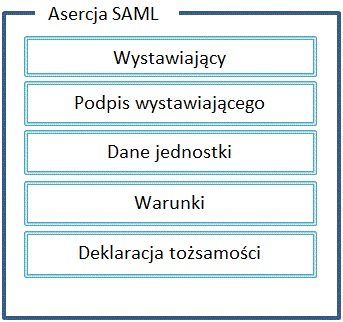
\includegraphics{img/samlAssertion.jpg}
				\caption{Elementy asercji SAML}
				\label{Elementy asercji SAML}
				\end{figure}

				Asercja SAML zawiera informacje o wystawiającym asercję. Może zawierać również informację o dacie wygenerowania asercji. W celu zapewnienia integralności informacji do asercji dołączany jest cyfrowy podpis wystawiającego. W dalszej części asercji znajdują się dane opisujące jednostkę, względem której utworzono asercję. Następną sekcją wiadomości są warunki, pod którymi asercja może być wykorzystywana. W tym fragmencie mogą znajdować się informacje o okresie ważności asercji lub usługi, do których adresowana jest asercja. Ostatnim elementem jest deklaracja tożsamości, zawierające informacje kontekstowe o procesie uwierzytelniania, np. dotyczące zastosowanej metody uwierzytelniania.

			\subparagraph{Typy deklaracji tożsamości}\mbox{}\\

				Dokument [31] definiuje następujące typy deklaracji tożsamości zawartych w asercjach SAML:

				\begin{itemize}
				  \item deklaracja uwierzytelniania - stwierdza, że opisana w asercji jednostka została uwierzytelniona w danym momencie przy użyciu mechanizmów opisanych w opisie kontekstu deklaracja
				  \item deklaracja atrybutu - stwierdza, że dany atrybut o zadanej wartości jest przypisany jednostce
				  \item deklaracja autoryzacji - stwierdza, że jednostce opisanej w asercji przyznano lub odmówiono praw dostępu do zasobów pod określonymi warunkami
				 \end{itemize}

		\paragraph{Protokoły}\mbox{}\\ 

			Protokoły SAML definiują format wiadomości żądań i odpowiedzi pozwalających na komunikację pomiędzy elementami systemu zarządzania tożsamościami przy pomocy technologii SAML. Specyfikacja SAML określa protokoły:

			\begin{itemize}
			  \item protokół odpytywania usługi "Identity Provider" o asercje
			  \item protokół żądania uwierzytelniania jednostki
			  \item protokół rejestrowania identyfikatorów jednostek
			  \item protokół żądania wygaśnięcia identyfikatora jednostki
			  \item protokół żądania jednokrotnego wylogowania z wielu aplikacji
			  \item protokół żądania odzwierciedlenia pomiędzy różnymi identyfikatorami jednostki
			\end{itemize}

		\paragraph{Mapowania dla protokołów komunikacyjnych}\mbox{}\\

			Mapowania SAML do protokołów komunikacyjnych określają w jaki sposób wiadomości protokołów SAML powinny być przekazywane przy pomocy standardowych protokołów komunikacyjnych.  Mapowania mogą np. definiować sposób przesyłania wiadomości SAML przy pomocy protokołów HTTP lub SOAP.

		\paragraph{Profile}\mbox{}\\

			Profile SAML definiują zbiór funkcjonalności jakie można uzyskać przy użyciu elementów niższych warstw(asercji, protokołów i mapowań) oraz sposób w jaki te funkcjonalności mogą być osiągnięte. Przykładem mogą być profile jednokrotnego uwierzytelniania specyfikujące sposób komunikacji pomiędzy dostawcami usług i serwisami "Identity Provider" w celu dostarczenia mechanizmów SSO lub profile zapytania o asercję dla jednostki.

\subsection{OpenID}

%---------------------------------------------------------------------------

\section{Przyklady frameworków zarzadzajacych autentykacja i autoryzacja uzytkowników}
\label{sec:frameworki}

Przyklady frameworków zarzadzajacych autentykacja i autoryzacja uzytkowników

%---------------------------------------------------------------------------
